%\documentclass[compress]{beamer}
\documentclass[8pt]{beamer}

%-----------------------------------------------------------
% PACKAGES

%\usepackage[latin1]{inputenc}
\mode<presentation>

%\usepackage[T1]{fontenc}  
%\usetheme{Warsaw}
\usetheme{Frankfurt}

\usepackage{graphicx}
%\usepackage[section]{placeins} % force � mettre l'image o� on veut
%\usepackage{float} %utiliser H pour forcer � mettre l'image o� on veut
\usepackage{lscape} %utilisation du mode paysage
%\usepackage{pslatex}
\usepackage{url}
\usepackage{subfigure}

\usepackage{graphicx}
\usepackage{tabls}
\usepackage{afterpage}

\usepackage{ocgx2}
\usepackage[]{media9}
%\usepackage{multimedia}

\usepackage{amsthm}
\usepackage{amssymb}
\usepackage{amsmath}
\usepackage{amsfonts}
\usepackage{amstext}
\usepackage{amsbsy}
\usepackage{mathbbol} 
\usepackage{mathrsfs}

\usepackage{epsfig}
%\usepackage{epsfig}
%\usepackage{cites}
\usepackage{epsf}
\usepackage{array}
\usepackage{color}
\usepackage{pdfpages}
\usepackage{cancel}

\usepackage{tikz}
%\usepackage{booktabs}

%-----------------------------------------------------------
% NEW  DEFINITIONS
%
%=================================================================================================
% new commands
% +++++++++++++++++++++++++++++++++++++++++++++++++++++++++++++++++++++++++++++++++++++++++++++++++
\newcommand{\nc}{\newcommand}
%
% Ways of grouping things
%
\newcommand{\bracket}[1]{\left[ #1 \right]}
\newcommand{\bracet}[1]{\left\{ #1 \right\}}
\newcommand{\fn}[1]{\left( #1 \right)}
\newcommand{\ave}[1]{\left\langle #1 \right\rangle}
%
% Derivative forms
% 
\newcommand{\dx}[1]{\,d#1}
\newcommand{\dxdy}[2]{\frac{\partial #1}{\partial #2}}
\newcommand{\dxdt}[1]{\frac{\partial #1}{\partial t}}
\newcommand{\dxdz}[1]{\frac{\partial #1}{\partial z}}
\newcommand{\dfdt}[1]{\frac{\partial}{\partial t} \fn{#1}}
\newcommand{\dfdz}[1]{\frac{\partial}{\partial z} \fn{#1}}
\newcommand{\ddt}[1]{\frac{\partial}{\partial t} #1}
\newcommand{\ddz}[1]{\frac{\partial}{\partial z} #1}
\newcommand{\dd}[2]{\frac{\partial}{\partial #1} #2}
\newcommand{\ddx}[1]{\frac{\partial}{\partial x} #1}
\newcommand{\ddy}[1]{\frac{\partial}{\partial y} #1}
%
% Vector forms
%
%\renewcommand{\vec}[1]{\ensuremath{\stackrel{\rightarrow}{#1}}}
%\renewcommand{\div}{\ensuremath{\vec{\nabla} \cdot}}
%\newcommand{\grad}{\ensuremath{\vec{\nabla}}}

\renewcommand{\div}{\vec{\nabla}\! \cdot \!}
\newcommand{\grad}{\vec{\nabla}}
\newcommand{\oa}[1]{\fn{\frac{1}{3}\hat{\Omega}\!\cdot\!\overrightarrow{A_{#1}}}}

%
% Equation beginnings and endings
%
\newcommand{\bea}{\begin{eqnarray}}
\newcommand{\eea}{\end{eqnarray}}
\newcommand{\be}{\begin{equation*}}
\newcommand{\ee}{\end{equation*}}
\newcommand{\beas}{\begin{eqnarray*}}
\newcommand{\eeas}{\end{eqnarray*}}
\newcommand{\bdm}{\begin{displaymath}}
\newcommand{\edm}{\end{displaymath}}
%
% Equation punctuation
% 
\newcommand{\pec}{\hspace{0.25in},}
\newcommand{\pep}{\hspace{0.25in}.}
\newcommand{\pev}{\hspace{0.25in}}
%
% Equation labels and references, figure references, table references
% 
\newcommand{\LEQ}[1]{\label{eq:#1}}
\newcommand{\EQ}[1]{Eq.~(\ref{eq:#1})}
\newcommand{\EQS}[1]{Eqs.~(\ref{eq:#1})}
\newcommand{\REQ}[1]{\ref{eq:#1}}
\newcommand{\LFI}[1]{\label{fi:#1}}
\newcommand{\FI}[1]{Fig.~\ref{fi:#1}}
\newcommand{\RFI}[1]{\ref{fi:#1}}
\newcommand{\LTA}[1]{\label{ta:#1}}
\newcommand{\TA}[1]{Table~\ref{ta:#1}}
\newcommand{\RTA}[1]{\ref{ta:#1}}

%
% List beginnings and endings
% 
\newcommand{\bl}{\bss\begin{itemize}}
\newcommand{\el}{\vspace{-.5\baselineskip}\end{itemize}\ess}
\newcommand{\benu}{\bss\begin{enumerate}}
\newcommand{\eenu}{\vspace{-.5\baselineskip}\end{enumerate}\ess}
%
% Figure and table beginnings and endings
% 
\newcommand{\bfg}{\begin{figure}}
\newcommand{\efg}{\end{figure}}
\newcommand{\bt}{\begin{table}}
\newcommand{\et}{\end{table}}
%
% Tabular and center beginnings and endings
% 
\newcommand{\bc}{\begin{center}}
\newcommand{\ec}{\end{center}}
\newcommand{\btb}{\begin{center}\begin{tabular}}
\newcommand{\etb}{\end{tabular}\end{center}}
%
% Single space command
% 
%\newcommand{\bss}{\begin{singlespace}}
%\newcommand{\ess}{\end{singlespace}}
\newcommand{\bss}{\singlespacing}
\newcommand{\ess}{\doublespacing}
%
%---New environment "arbspace". (modeled after singlespace environment
%                                in Doublespace.sty)
%   The baselinestretch only takes effect at a size change, so do one.
% 
\def\arbspace#1{\def\baselinestretch{#1}\@normalsize}
\def\endarbspace{}
\newcommand{\bas}{\begin{arbspace}}
\newcommand{\eas}{\end{arbspace}}
%
% An explanation for a function
%
\newcommand{\explain}[1]{\mbox{\hspace{2em} #1}}
%
% Quick commands for symbols
%  
\newcommand{\half}{\frac{1}{2}}
\newcommand{\third}{\frac{1}{3}}
\newcommand{\twothird}{\frac{2}{3}}
\newcommand{\fourth}{\frac{1}{4}}
\newcommand{\mdot}{\dot{m}}
\newcommand{\ten}[1]{\times 10^{#1}\,}
\newcommand{\cL}{{\cal L}}
\newcommand{\cD}{{\cal D}}
\newcommand{\cF}{{\cal F}}
\newcommand{\cE}{{\cal E}}
\renewcommand{\Re}{\mbox{Re}}
\newcommand{\Ma}{\mbox{Ma}}
%
% Inclusion of Graphics Data
%
%\input{psfig}
%\psfiginit
%
% More Quick Commands
% 
\newcommand{\bi}{\begin{itemize}}
\newcommand{\ei}{\end{itemize}}
\newcommand{\ben}{\begin{enumerate}}
\newcommand{\een}{\end{enumerate}}
\newcommand{\dxi}{\Delta x_i}
\newcommand{\dyj}{\Delta y_j}
\newcommand{\ts}[1]{\textstyle #1}


\newcommand{\bu}{\boldsymbol{u}}
\newcommand{\ber}{\boldsymbol{e}}
\newcommand{\br}{\boldsymbol{r}} 
\newcommand{\bo}{\boldsymbol{\Omega}}

\newcommand{\bn}{\boldsymbol{\nabla}}

% DGFEM commands
\newcommand{\jmp}[1]{[\![#1]\!]}                     % jump
\newcommand{\mvl}[1]{\{\!\!\{#1\}\!\!\}}             % mean value


\newcommand{\boxedeqn}[1]{%
  \[\fbox{%
      \addtolength{\linewidth}{-2\fboxsep}%
      \addtolength{\linewidth}{-2\fboxrule}%
      \begin{minipage}{\linewidth}%
      \begin{equation}#1\end{equation}%
      \end{minipage}%
    }\]%
}
\newcommand{\mboxed}[1]{\boxed{\phantom{#1}}}
\newcommand{\ud}{\,\mathrm{d}}

% keff
\newcommand{\keff}{\ensuremath{k_{\textit{eff}}}}

% margin par
\newcommand{\mt}[1]{\marginpar{ {\footnotesize #1} }}

% shortcut for aposterio in italics
\newcommand{\apost}{\textit{a posteriori\xspace}}
\newcommand{\Apost}{\textit{A posteriori}\xspace}

% shortcut for multi-group
\newcommand{\mg}{multigroup\xspace}
\newcommand{\Mg}{Multigroup\xspace}
\newcommand{\ho}{higher-order\xspace}
\newcommand{\Ho}{Higher-order\xspace}
\newcommand{\HO}{Higher-Order\xspace}
\newcommand{\HObig}{HIGHER-ORDER\xspace}
\newcommand{\Mgbig}{MULTIGROUP\xspace}

% shortcut for domain notation
\newcommand{\D}{\mathcal{D}}

% shortcut for xuthus
\newcommand{\psc}[1]{{\sc {#1}}}
\newcommand{\xuthus}{\psc{xuthus}\xspace}

% vector shortcuts
\newcommand{\vo}{\vec{\Omega}}
\newcommand{\vr}{\vec{r}}
\newcommand{\vn}{\vec{n}}
\newcommand{\vnk}{\vec{\mathbf{n}}}

% extra space
\newcommand{\qq}{\quad\quad}

% sign function
\DeclareMathOperator{\sgn}{sgn}


\newcommand{\ensuretext}[1]{\ensuremath{\text{#1}}}

% common reference commands
\newcommand{\eqt}[1]{Eq.~(\ref{#1})}                     % equation
\newcommand{\fig}[1]{Fig.~\ref{#1}}                      % figure
\newcommand{\tbl}[1]{Table~\ref{#1}}                     % table



\newcommand{\rhs}{right-hand-side\xspace}
\newcommand{\clearemptydoublepage}{\newpage{\pagestyle{empty}\cleardoublepage}}


\newcommand{\bs}[1]{\mathbf{#1}}
\renewcommand{\bs}[1]{\vec{#1}}
%\newcommand{\dd}{\mathrm{d}}
\newcommand{\norm}{\textrm{norm}}
\renewcommand{\Re}{\textrm{Re}}
\newcommand{\Pe}{\textrm{P\'e}}
\renewcommand{\Pr}{\textrm{Pr}}

\newcommand{\resi}{R_e}
%\newcommand{\resinew}{\tilde{D}_e}
\newcommand{\resinew}{\widetilde{\resi}}
\newcommand{\matder}[1]{\frac{\textrm{D} #1}{\textrm{D} t}}

\newcommand{\divv}[1]{\vec{\nabla}^{#1}\! \cdot \!}
\newcommand{\gradd}[1]{\vec{\nabla}^{#1}}

\newcommand{\tcr}[1]{\textcolor{red}{#1}}
\newcommand{\tcb}[1]{\textcolor{blue}{#1}}
\newcommand{\tcm}[1]{\textcolor{magenta}{#1}}
\newcommand{\tcp}[1]{\textcolor{violet}{#1}}

\renewcommand{\L}{\mathbf{L}}
\renewcommand{\S}{\mathbf{\Sigma}}
\newcommand{\M}{\mathbf{M}}
\renewcommand{\D}{\mathbf{D}}
%=================================================================================================

%============================================================

%style et couleur
%\usetheme{Frankfurt}
\date{\today}

%\addtobeamertemplate{footline}{\hfill\insertframenumber/\inserttotalframenumber\hspace{2em}\null}

\setbeamertemplate{footline}{
\leavevmode%
%\hbox{\hspace*{-0.06cm}
\begin{beamercolorbox}[wd=.5\paperwidth,ht=3.25ex,dp=1ex,center]{author in head/foot}%
	\usebeamerfont{author in head/foot}\insertshortauthor%~~(\insertshortinstitute)
\end{beamercolorbox}%
\begin{beamercolorbox}[wd=.25\paperwidth,ht=3.25ex,dp=1ex,center]{section in head/foot}%
	\usebeamerfont{section in head/foot} IQS PHYSOR 2016 % \insertshorttitle
\end{beamercolorbox}%
\begin{beamercolorbox}[wd=.25\paperwidth,ht=3.25ex,dp=1ex,left]{section in head/foot}%
	\usebeamerfont{section in head/foot}\insertshortdate{}\hspace*{2em}
	\insertframenumber{} / \inserttotalframenumber %\hspace*{2ex}
\end{beamercolorbox}}%
%\vskip0pt%
%}

\beamertemplatetransparentcovered

\urldef{\ragusa}\url{jean.ragusa@tamu.edu}
\urldef{\prince}\url{zachmprince@tamu.edu}

\title{Improved Quasi-Static Method in Rattlesnake}

\author{Zachary M. Prince$^*$, Jean C. Ragusa$^*$, Yaqi Wang$^{\dagger}$}
\institute{$^*$Department of Nuclear Engineering, Texas A\&M University, College Station, TX \\ $^\dagger$Idaho National Lab , Idaho Falls, ID}

%%%%%%%%%%%%%%%%%%%%%%%%%%%%%%%%%%%%%%%%%%%%%%%%%%%%%%%%%%%%%%%%%%%%

%%%%%%%%%%%%%%%%%%%%%%%%%%%%%%%%%%%%%%%%%%%%%%%%%%%%%%%%%%%%%%%%%%%%
%%%%%%%%%%%%%%%%%%%%%%%%%%%%%%%%%%%%%%%%%%%%%%%%%%%%%%%%%%%%%%%%%%%%
\begin{document}
%%%%%%%%%%%%%%%%%%%%%%%%%%%%%%%%%%%%%%%%%%%%%%%%%%%%%%%%%%%%%%%%%%%%
%%%%%%%%%%%%%%%%%%%%%%%%%%%%%%%%%%%%%%%%%%%%%%%%%%%%%%%%%%%%%%%%%%%%

%-------------------------------------------------------------------
\begin{frame}
\vspace{-1.5cm}
	\begin{figure}[t]
		\centering
			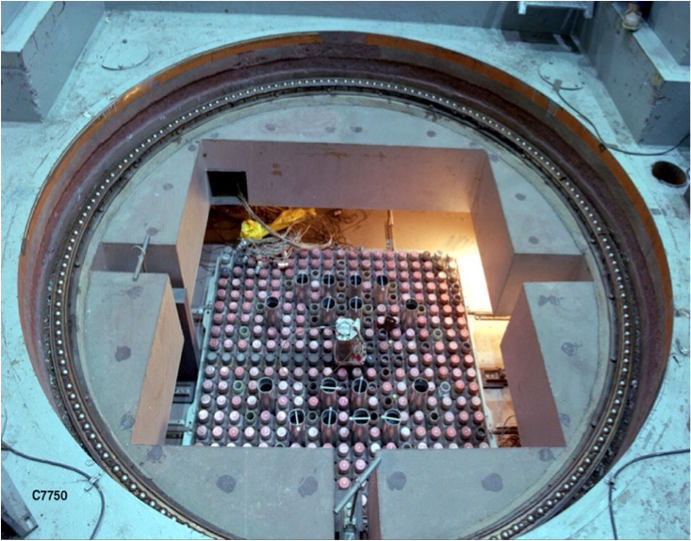
\includegraphics[width=.45\textwidth]{figures/Treat_core_view.png}
	\end{figure}
\vspace{-0.5cm}
\titlepage
\vspace{-0.5cm}
\small{email: {\prince} }

\end{frame}
%-------------------------------------------------------------------

%-------------------------------------------------------------------
\begin{frame}
	\frametitle{Outline}
	\tableofcontents 
\end{frame}
%-------------------------------------------------------------------

%%%%%%%%%%%%%%%%%%%%%%%%%%%%%%%%%%%%%%%%%%%%%%%%%%%%%%%%%%%%%%%%%%%%
%%%%%%%%%%%%%%%%%%%%%%%%%%%%%%%%%%%%%%%%%%%%%%%%%%%%%%%%%%%%%%%%%%%%
\section{Theory}
%%%%%%%%%%%%%%%%%%%%%%%%%%%%%%%%%%%%%%%%%%%%%%%%%%%%%%%%%%%%%%%%%%%%
%%%%%%%%%%%%%%%%%%%%%%%%%%%%%%%%%%%%%%%%%%%%%%%%%%%%%%%%%%%%%%%%%%%%

%%%%%%%%%%%%%%%%%%%%%%%%%%%%%%%%%%%%%%%%%%%%%%%%%%%%%%%%%%%%%%%%%%%%
\subsection{Time-dependent Multigroup Diffusion}
%%%%%%%%%%%%%%%%%%%%%%%%%%%%%%%%%%%%%%%%%%%%%%%%%%%%%%%%%%%%%%%%%%%%

%-------------------------------------------------------------------
\begin{frame}{Time-dependent Multigroup Diffusion}

\vspace{-3mm}

\begin{block}{Group Fluxes $\phi^g$ $(1 \le g \le G )$ with Precursors $C_i$ $(1 \le i \le I)$}
\begin{align*}
\frac{1}{v^g} \frac{\partial \phi^g }{\partial t} =& \frac{\chi_p^g}{\keff} \sum_{g'=1}^G (1-\beta) \nu^{g'} \Sigma_f^{g'} \phi^{g'} -  \left( -\div D^g \grad  + \Sigma_r^g \right) \phi^g  \nonumber \\
&  + \sum_{g'\neq g}^G\Sigma_s^{g'\to g} \phi^{g'}  + \sum_{i=1}^I\chi_{d,i}^g\lambda_i C_i \ , \quad 1 \le g \le G 
\end{align*}
\be
\frac{dC_i}{dt} = \frac{\beta_i}{k_{eff}}\sum_{g=1}^G\nu^{g} \Sigma_f^g \phi^{g} - \lambda_i C_i \ , \quad 1 \le i \le I 
\ee
\end{block}

%\vspace{-4mm}

\begin{block}{Flux Factorization}
Decomposition of the multigroup flux into the product of a time-dependent \tcr{amplitude} ($\tcr{p}$) and a space-/time-dependent multigroup \tcb{shape} ($\tcb{\varphi^g}$):
\begin{equation*}
\phi^g(\vec{r},t) = \tcr{p(t)} \tcb{\varphi^g(\vec{r},t)}
\end{equation*}

\begin{itemize}
\item 
Factorization is \textbf{not} an approximation.
\item
Note that $\tcr{p(t)}$ and $\tcb{\varphi^g(\vec{r},t)}$ are not unique. 
%\[
%\phi= \tcr{p} \times \tcb{\psi} = \tcr{\frac{p}{a}} \times \tcb{\left( a \psi \right)}
%\]
\end{itemize}
\end{block}
%--------------

\end{frame}
%-------------------------------------------------------------------


%%%%%%%%%%%%%%%%%%%%%%%%%%%%%%%%%%%%%%%%%%%%%%%%%%%%%%%%%%%%%%%%%%%%
\subsection{IQS equations}
%%%%%%%%%%%%%%%%%%%%%%%%%%%%%%%%%%%%%%%%%%%%%%%%%%%%%%%%%%%%%%%%%%%%

%-------------------------------------------------------------------
\begin{frame}{Shape equations}

\begin{block}{Shape equations}
Implementing factorization and solving for $\tcb{\varphi^g}$:
\begin{align*}
\frac{1}{v^g} \frac{\partial \tcb{\varphi^g} }{\partial t} =& \frac{\chi_p^g}{\keff} \sum_{g'=1}^G (1-\beta) \nu^{g'} \Sigma_f^{g'} \tcb{\varphi^{g'}} -  \left( -\div D^g \grad  + \Sigma_r^g + \tcr{\frac{1}{v^g}}\tcr{\frac{1}{p}}\tcr{\frac{dp}{dt}}\right) \tcb{\varphi^g}  \nonumber \\
&  + \sum_{g'\neq g}^G\Sigma_s^{g'\to g} \tcb{\varphi^{g'}}  + \tcr{\frac{1}{p}}\sum_{i=1}^I\chi_{d,i}^g\lambda_i C_i \ , \quad 1 \le g \le G 
\end{align*}
\begin{equation*}
\frac{dC_i}{dt} = \tcr{p}\sum_{g=1}^G \nu_{d,i} \Sigma_f^g \tcb{\varphi^{g}} - \lambda_iC_i , \quad 1 \le i \le I
\end{equation*}
%\be
%\frac{dC_i}{dt} = \frac{\beta_i}{k_{eff}}\sum_{g=1}^G\nu^{g} \Sigma_f^g \tcr{p} \varphi^{g} - \lambda_i C_i \ , \quad 1 \le i \le I 
%\ee
\end{block}

\begin{block}{Differences with original transport equation}
\ben
\item An additional removal term based on $\tcr{\frac{1}{v^g}\frac{1}{p}\frac{dp}{dt}} \tcb{\psi^g}$
\item Delayed neutron source term scaled by $\tcr{\frac{1}{p}}$
\item The delayed fission source in the precursor equation scaled by \tcr{p}
\een
\end{block}

\end{frame}
%-------------------------------------------------------------------

%%%%%%%%%%%%%%%%%%%%%%%%%%%%%%%%%%%%%%%%%%%%%%%%%%%%%%%%%%%%%%%%%%%%
% \subsection{Amplitude equations}
%%%%%%%%%%%%%%%%%%%%%%%%%%%%%%%%%%%%%%%%%%%%%%%%%%%%%%%%%%%%%%%%%%%%


%-------------------------------------------------------------------
\begin{frame}{Amplitude equations (PRKE)}

\begin{block}{Principle}
To obtain the \tcr{amplitude} equation, we multiply the shape equations with a weighting 
function (initial adjoint flux, $\phi^{*g}$), then integrate over domain.  
\end{block}

\begin{block}{Notation}
For brevity, the adjoint flux product and integration over domain will be represented with parenthetical notation:
\[
\int_D\phi^{*g}(\vec{r})f(\vec{r})dr^3=\left(\phi^{*g},f\right)
\]
\end{block}


\begin{block}{Uniqueness of the factorization}
In order to impose uniqueness of the factorization, one requires:
\[
\tcp{K_0} = \sum_{g=1}^G\left(\phi^{*g},\frac{1}{v^g}\varphi^g\right)= constant
\]
\tcm{This condition will be the criteria for solution convergence}
\end{block}


\end{frame}
%-------------------------------------------------------------------

%-------------------------------------------------------------------
\begin{frame}{Point Reactor Kinetics Equation}
\vspace{-2mm}
\begin{block}{PRKE}
\[
\frac{d\tcr{p}}{dt}=\left[\frac{\rho-\bar{\beta}}{\Lambda}\right]\tcr{p}+\sum_{i=1}^I\bar{\lambda}_i\xi_i
\]
\[
\frac{d\xi_i}{dt}=\frac{\bar{\beta}_i}{\Lambda}\tcr{p} - \bar{\lambda}_i\xi_i \quad 1 \le i \le I 
\]
\end{block}
\vspace{-3mm}
\begin{block}{PRKE Coefficients}

\small \be
\frac{\rho-\bar{\beta}}{\Lambda}=
\frac{ \sum_{g=1}^G \left(\phi^{*g},\sum_{g'=1}^G\frac{\chi_p^g}{\keff} \nu_p^{g'} \Sigma_f^{g'}\varphi^{g'} + \sum_{g'\neq g}^G\Sigma_s^{g'\to g} \varphi^{g'} -\left( -\div D^g \grad  + \Sigma_r^g \right)\varphi^g\right)}
{\sum_{g=1}^G \left(\phi^{*g},\frac{1}{v^g}\varphi^g\right)}
\ee \normalsize
%%
\be
\frac{\bar{\beta}}{\Lambda}=\sum_{i=1}^I\frac{\bar{\beta}_i}{\Lambda}=\frac{1}{\keff}
\frac{\sum_{i=1}^I\sum_{g=1}^G(\phi^{*g}, \beta_i\nu^{g} \Sigma_f^g \varphi^{g})}
{\sum_{g=1}^G \left(\phi^{*g},\frac{1}{v^g}\varphi^g\right)}
\ee
%%
\be
\bar{\lambda}_i=\frac{\sum_{g=1}^G(\phi^{*g},\chi_{d,i}^g\lambda_i C_i)}{\sum_{g=1}^G(\phi^{*g},\chi_{d,i}^gC_i)}
\ee
\tcm{These functionals seem daunting to implement but this was relatively straightforward with a couple of options available in MOOSE: (1) element integral postprocessors and (2) {\tt save\_in} kernel attributes)}
\end{block}

\end{frame}
%-------------------------------------------------------------------

%-------------------------------------------------------------------
%\begin{frame}{Shape equations: Implementation within the MOOSE framework}
%
%\begin{block}{Shape equations $\to$ \tcm{FEM solver + implicit time integration}}
%\begin{equation*}
%\boxed{
%\frac{1}{v}\frac{\tcb{\psi}^{n+1}-\tcb{\psi}^n }{\Delta t} = \left(H^{n+1} + P_p^{n+1} - L^{n+1} -\tcr{\frac{1}{v}\frac{1}{p^{n+1}}\left.\frac{dp}{dt}\right|_{n+1}} \right) \tcb{\psi}^{n+1}  + \tcr{\frac{1}{p^{n+1}}} S_{d}^{n+1} 
%}
%\end{equation*}
%\end{block}
%
%\begin{block}{Modification to the original transport equation}
%\ben
%\item An additional removal term based on $\tcr{\frac{1}{v^g}\frac{1}{p}\frac{dp}{dt}} \tcb{\psi^g}$\\
%\tcm{$\to$ add a new kernel in Rattlesnake} (easy)
%\item Delayed neutron source term scaled by $\tcr{\frac{1}{p}}$\\
%\tcm{$\to$ scale the delayed neutron source kernel} (easy)
%\item nonlinear coupling between shape variable $\tcb{\psi^{n+1}}$ and amplitude variable $\tcr{p^{n+1}}$\\
%\tcm{$\to$ employ MOOSE's nonlinear solvers} (easy)
%\een
%\end{block}
%
%\end{frame}
%-------------------------------------------------------------------


%%%%%%%%%%%%%%%%%%%%%%%%%%%%%%%%%%%%%%%%%%%%%%%%%%%%%%%%%%%%%%%%%%%%
\subsection{IQS method solution process}
%%%%%%%%%%%%%%%%%%%%%%%%%%%%%%%%%%%%%%%%%%%%%%%%%%%%%%%%%%%%%%%%%%%%

%-------------------------------------------------------------------
\begin{frame}{IQS}

\begin{block}{Factorization leads to a nonlinear system}
The \tcr{amplitude} and \tcb{shape} equations form a system of nonlinear coupled equations: 
\ben
\item the coefficients appearing in the \tcr{PRKE}'s depend upon the \tcb{shape} solution,
\item the \tcb{shape} equation has a kernel dependent on \tcr{amplitude} and its derivative,  
%\item the delayed neutron source term is scaled by the amplitude.
\een
\end{block}

\begin{block}{Time scales and IQS method solution process}
Because solving for the \tcb{shape} can be expensive, especially in two or three dimensions, it is attractive to make the assumption that the \tcb{shape} is weakly time-dependent so the \tcb{shape} can be computed after a multitude of \tcr{PRKE} calculations:
%

\begin{figure}[h]
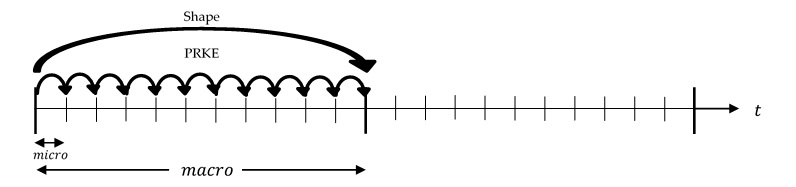
\includegraphics[width=\linewidth]{figures/IQS_visualization.jpg}
%\caption{IQS method solution process}
\label{fig:IQS}
\end{figure}

\tcm{In MOOSE, we employ the available Picard iteration functionality to resolve the nonlinearities}
\end{block}
\end{frame}
%-------------------------------------------------------------------

%-------------------------------------------------------------------
\begin{frame}{Convergence criteria}


\begin{block}{Ideally}
The normalization constant should not change over time !
\[
\tcp{K_0} = \sum_{g=1}^G\left(\phi^{*g},\frac{1}{v^g}\varphi^g_0\right)= constant
\]
\[
\text{Thus, we employ }\quad
\left| \frac{\sum_{g=1}^G\left(\phi^{*g},\frac{1}{v^g}\varphi^g_{n+1}\right)}{\tcp{K_0}}-1\right| 
= \left| \frac{\tcp{K_{n+1}}}{{\tcp{K_0}}}-1\right|  < tol
\]
\end{block}

\begin{block}{Note that we have seen in practice ... }
\[
\frac{ \| \varphi^{g,\tcr{\ell+1}}_{n+1} - \varphi^{g,\tcr{\ell}}_{n+1} \|}{\| \varphi^{g,\tcr{\ell+1}}_{n+1} \|} < tol 
\quad \text{or even} \quad
\frac{ \| \varphi^{g,\tcr{\ell+1}}_{n+1} - \varphi^{g,\tcr{0}}_{n+1} \|}{\| \varphi^{g,\tcr{0}}_{n+1} \|} < tol 
\]
where $\tcr{\ell}$ is the IQS iteration index over a given macro time step $[t_n,t_{n+1}]$\\
\smallskip
These empirical criteria must be followed by a renormalization before starting the next time step $[t_{n+1},t_{n+2}]$
\[
 \varphi^{g,\tcr{converged}}_{n+1} \times \frac{\tcp{K_{n+1}^{\tcr{converged}}}}{\tcp{K_0}} \rightarrow \varphi^{g}_{n+1}
\]
\end{block}


\end{frame}
%-------------------------------------------------------------------

%-------------------------------------------------------------------
\begin{frame}{IQS Predictor-Corrector}

%\begin{block}{IQS P-C Linearizes the System}
IQS P-C linearizes the system and avoids iterations on the \tcb{shape}: 
\ben
\item Evaluate multigroup diffusion equation to get predicted flux $\phi_{n+1}^{g,\tcr{pred}}$
\item Scale predicted flux to obtain \tcb{shape}:
\[
\tcb{\varphi^{g}_{n+1}} = \phi_{n+1}^{g,\tcr{pred}} \frac{\sum_{g=1}^G\left(\phi^{*g},\frac{1}{v^g}\varphi^g_{n+1}\right)}{\sum_{g=1}^G \left(\phi^{*g},\frac{1}{v^g}\phi_{n+1}^{g,\tcr{pred}}\right)} = \phi_{n+1}^{g,\tcr{pred}} \frac{\tcp{K_0}}{\tcp{K_{n+1}}}
\]
\item Compute PRKE parameters at $t_{n+1}$
\item Evaluate PRKE along micro step using interpolated parameters to obtain $\tcr{p_{n+1}}$
\item Scale $\tcb{\varphi^{g}_{n+1}}$ to obtain corrected flux:
\[
\phi_{n+1}^{g,\tcr{corr}} = \tcr{p_{n+1}} \times \tcb{\varphi^{g}_{n+1}}
\]
\een

 Advantage: No IQS nonlinear iteration is necessary \\
 Disadvantage: Assumes $\sum_{g=1}^G\left(\phi^{*g},\frac{1}{v^g}\varphi^g_{n+1}\right)$ is inherently constant \\
\vspace{2mm}
\small \tcm{Note: The PRKE parameters can be computed using flux since the amplitude is in the numerator and denominator of each one. So Step 2 is unnecessary if the corrected flux is solved with}:
\[
\phi_{n+1}^{g,\tcr{corr}} = \phi_{n+1}^{g,\tcr{pred}} \times \frac{\tcp{K_0}}{\tcp{K_{n+1}}} \tcr{p_{n+1}}
\]
\normalsize
%\end{block}

\end{frame}
%-------------------------------------------------------------------

%%%%%%%%%%%%%%%%%%%%%%%%%%%%%%%%%%%%%%%%%%%%%%%%%%%%%%%%%%%%%%%%%%%%%
%\subsection{Precursors time-discretization}
%%%%%%%%%%%%%%%%%%%%%%%%%%%%%%%%%%%%%%%%%%%%%%%%%%%%%%%%%%%%%%%%%%%%%
%
%%-------------------------------------------------------------------
%\begin{frame}{Precursors time-discretization}
%
%A simple ODE:
%\begin{equation*}
%\boxed{
%\frac{dC_i}{dt} = \sum_{g=1}^G \nu_{d,i} \Sigma_f^g(\vec{r},t) \tcr{p} \tcb{\varphi^{g}}(\vec{r},t) - \lambda_i(\vec{r},t) C_i(\vec{r},t) 
%}
%\end{equation*}
%\begin{block}{Numerical integration: Theta-scheme (already in Rattlesnake)}
%\be
%C^{n+1} = \frac{1-(1-\theta)\Delta t\lambda}{1+\theta\Delta t\lambda}C^n 
%+ \frac{(1-\theta)\Delta t \beta (\nu\Sigma_f)^n}    {1+\theta\Delta t\lambda}\tcb{\varphi^n}     \tcr{p^n }
%+ \frac{\theta\Delta t     \beta (\nu\Sigma_f)^{n+1}}{1+\theta\Delta t\lambda}\tcb{\varphi^{n+1}} \tcr{p^{n+1}}
%\ee
%Reporting this value of $C^{n+1}$ in $S_d^{n+1}$, one can solve for the shape $\psi^{n+1}$ as a function of $\psi^n$ and $C^n$
%(and $p^n$, $p^{n+1}$, $dp/dt|_n$ and  $dp/dt|_{n+1}$).\\
%
%\bigskip
%Once $\psi^{n+1}$ has been determined, $C^{n+1}$ is updated. \\
%
%\medskip
%Rattlesnake currently implements both implicit ($\theta=1$) and Crank-Nicholson ($\theta=1/2$) as options for precursor evaluation.
%
%\end{block}
%
%\end{frame}
%%-------------------------------------------------------------------
%
%%-------------------------------------------------------------------
%\begin{frame}{Analytical Integration}
%
%
%\begin{block}{Analytical Integration}
%\[
%C^{n+1} =  C^n e^{-\lambda (t_{n+1} - t_n) }  + \int_{t_n}^{t_{n+1}} \nu_d\Sigma_f(t')\tcb{\varphi(t')} \tcr{p(t')} e^{-\lambda (t_{n+1}-t')}dt'
%\]
%\end{block}
%
%\begin{block}{}
%Assuming a \tcb{linear in time variation} over the macro time step $[t_n, t_{n+1}]$ for the \tcb{shape} and the \tcb{fission cross section}, we get:
%\[
%C^{n+1} = C^n e^{-\lambda \Delta t} 
%+ \left[\tcm{a_3}(\nu_d\Sigma_f)^{n+1}+\tcm{a_2}(\nu_d\Sigma_f)^n\right]\tcb{\varphi^{n+1}}
%+ \left[\tcm{a_2}(\nu_d\Sigma_f)^{n+1}+\tcm{a_1}(\nu_d\Sigma_f)^n\right]\tcb{\varphi^n    }
%\]
%where the integration coefficients are defined as:
%\begin{align}
%&a_1 = \int_{t_n}^{t_{n+1}}\left(\frac{t_{n+1}-t'}{\Delta t}\right)^2 \tcr{p(t')} e^{-\lambda(t_{n+1}-t')}dt' \notag \\
%&a_2= \int_{t_n}^{t_{n+1}}\frac{(t'-t_n)(t_{n+1}-t')}{(\Delta t)^2}   \tcr{p(t')} e^{-\lambda(t_{n+1}-t')}dt'   \notag \\
%&a_3 = \int_{t_n}^{t_{n+1}}\left(\frac{t'-t_n}{\Delta t}\right)^2     \tcr{p(t')} e^{-\lambda(t_{n+1}-t')}dt'     \notag 
%\end{align}
%
%
%The amplitude $\tcr{p}$ is contained in the $a_i$'s integration coefficients.\\
%\tcr{$p(t)$} has been \tcm{accurately} calculated at the \tcm{micro time} step level.
%
%\end{block}
%
%\end{frame}
%%-------------------------------------------------------------------
%
%%%-------------------------------------------------------------------
%%\begin{frame}{Analytical Integration (continued)}
%%
%%Recall that we just need to compute  coefficients of the form:
%%\[
%%\int_{t_n}^{t_{n+1}}\left(\delta_2 t'^2 + \delta_1 t' +\delta_0\right) \tcr{p(t')}e^{-\lambda(t_{n+1}-t')}dt' 
%%\]
%%
%%\begin{block}{}
%%
%%The amplitude $(p)$ is contained in the $a_i$'s integration coefficients.\\
%%$p(t)$ has been highly accurately calculated at the micro time step level.
%%
%%\end{block}
%%
%%\end{frame}
%%%-------------------------------------------------------------------

%%%%%%%%%%%%%%%%%%%%%%%%%%%%%%%%%%%%%%%%%%%%%%%%%%%%%%%%%%%%%%%%%%%%
%%%%%%%%%%%%%%%%%%%%%%%%%%%%%%%%%%%%%%%%%%%%%%%%%%%%%%%%%%%%%%%%%%%%
\section{Rattlesnake Implementation}
%%%%%%%%%%%%%%%%%%%%%%%%%%%%%%%%%%%%%%%%%%%%%%%%%%%%%%%%%%%%%%%%%%%%
%%%%%%%%%%%%%%%%%%%%%%%%%%%%%%%%%%%%%%%%%%%%%%%%%%%%%%%%%%%%%%%%%%%%

\subsection{Changes to Rattlesnake}

%-------------------------------------------------------------------
\begin{frame}{Changes to Rattlesnake}
\vspace{-2mm}
\begin{block}{Action Systems}
\bi
\item Continuous FEM Diffusion (\tcm{almost complete})
\item Discontinuous FEM Diffusion 
\item Discontinuous FEM Sn Transport (first-order form) 
\item Discontinuous FEM Sn Transport (SAAF form)
\ei
Four action systems \tcr{$\ne$} four times the work!
\end{block}
\vspace{-2mm}
\begin{block}{Break down of IQS Changes}
\begin{figure}[h]
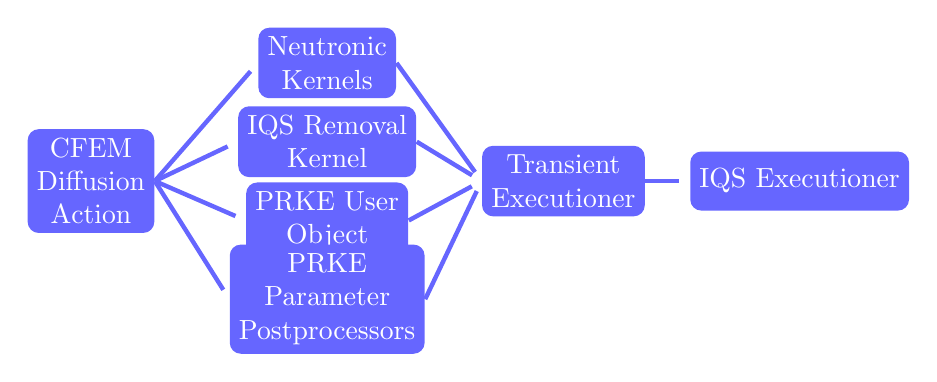
\begin{tikzpicture}[every node/.style = {shape          = rectangle, rounded corners, fill = blue!60, minimum width  = 1.5cm, minimum height = 0.75cm, align= center, text = white},blue edge/.style  = { -, ultra thick, blue!60, shorten >= 4pt}]
\node(0;0) at (-1,0) {CFEM \\ Diffusion \\ Action};
  \node(1;3)  at (2, 1.5) {Neutronic \\ Kernels};   
  \node(1;1)  at (2, 0.5) {IQS Removal \\ Kernel}; 
  \node(1;-1)  at (2,-0.5) {PRKE User \\ Object}; 
  \node(1;-3) at (2,-1.5) {PRKE \\ Parameter \\ Postprocessors}; 
     \node(2;0)  at (5,0) {Transient \\ Executioner};
     	\node(3;0)  at (8,0) {IQS Executioner};
\foreach \j in {-3,-1,1,3}
  { \draw[blue edge] (0;0.east) -- (1;\j.west); }
\foreach \j in {-3,-1,1,3}
  { \draw[blue edge] (1;\j.east) -- (2;0.west);} 
\draw[blue edge] (2;0.east) -- (3;0.west);         
\end{tikzpicture}
%\caption{CFEM Diffusion Action Process Diagram}   
\label{Action}
\end{figure}
\end{block}

%\begin{block}{}
%\bi
%\item \tcm{Action System} (adding IQS as an option)
%\item Post-processors (\tcm{element integrals}) for PRKE coefficients: $\rho-\bar{\beta}$, $\bar{\beta}_i$, $\bar{\lambda}_i$\\
%Note that the numerator of $\rho-\bar{\beta}$, i.e., $\left( \Psi^{*}, (H+P_p-L) \psi \right)$, is particularly easy thanks to the residual {\tt save\_in} option of MOOSE.
%\item IQS \tcm{userobject} (PRKE solve using updated PRKE coefficients)
%\item IQS \tcm{executioner} derived from MOOSE executioner (use of the existing Picard iteration loop in the {\tt transient} executioner; this can seamlessly enable IQS in multiphysics simulations without any further changes)
%\ei
%\end{block}

\end{frame}
%-------------------------------------------------------------------


%-------------------------------------------------------------------
\begin{frame}{Changes for Shape and PRKE Parameters}

\begin{block}{Kernels}
\bi
\item Addition of IQS removal kernel that evaluates $\tcr{\frac{1}{v^g}\frac{1}{p}\frac{dp}{dt}} \tcb{\varphi^g}$ residual
\item Modification of precursor kernel so that delayed source is scaled by $\tcr{\frac{1}{p}}$
\ei
\end{block}

\begin{block}{Post-Processors}
\bi
\item Numerators of $\bar{\beta}_i$ and $\bar{\lambda}_i$, as well as the denominator $\Lambda$ are evaluated by transferring material properties and performing an element integral
\item The terms of the $\rho-\bar{\beta}$ numerator are residuals of various kernels. These residuals are saved into a variable using MOOSE \texttt{save\_in} functionality.  The the inner product of this variable and the adjoint solution is then evaluated.
\item A user-object is used to perform divisions of post-processor values and passes them to the executioner
\ei

\end{block}

\end{frame}
%-------------------------------------------------------------------

%-------------------------------------------------------------------
\begin{frame}{Executioner}

\begin{block}{IQS}
\ben
\item \tcr{PRKE} evaluation using SDIRK33 time integration
\item Perform \tcb{shape} evaluation
\item Re-evaluate $\tcp{\sum_{g=1}^G\left(\phi^{*g},\frac{1}{v^g}\varphi^g\right)}$ for IQS error criteria
\item Iterate \tcr{PRKE} and \tcb{shape} evaluation using Picard iteration functionality
\een
\end{block}

\begin{block}{IQS P-C}
\ben
\item Flux evaluation
\item \tcr{PRKE} evaluation using SDIRK33 time integration
\item Scale predicted flux
\item Re-evaluate precursors with corrected flux
\een
\end{block}


\end{frame}
%-------------------------------------------------------------------

%%%%%%%%%%%%%%%%%%%%%%%%%%%%%%%%%%%%%%%%%%%%%%%%%%%%%%%%%%%%%%%%%%%%
%%%%%%%%%%%%%%%%%%%%%%%%%%%%%%%%%%%%%%%%%%%%%%%%%%%%%%%%%%%%%%%%%%%%
\section{Results}
%%%%%%%%%%%%%%%%%%%%%%%%%%%%%%%%%%%%%%%%%%%%%%%%%%%%%%%%%%%%%%%%%%%%
%%%%%%%%%%%%%%%%%%%%%%%%%%%%%%%%%%%%%%%%%%%%%%%%%%%%%%%%%%%%%%%%%%%%

%%%%%%%%%%%%%%%%%%%%%%%%%%%%%%%%%%%%%%%%%%%%%%%%%%%%%%%%%%%%%%%%%%%
\subsection{1D Test Case}
%%%%%%%%%%%%%%%%%%%%%%%%%%%%%%%%%%%%%%%%%%%%%%%%%%%%%%%%%%%%%%%%%%%

%-------------------------------------------------------------------
\begin{frame}{1D Test Case}

\begin{figure}[h]
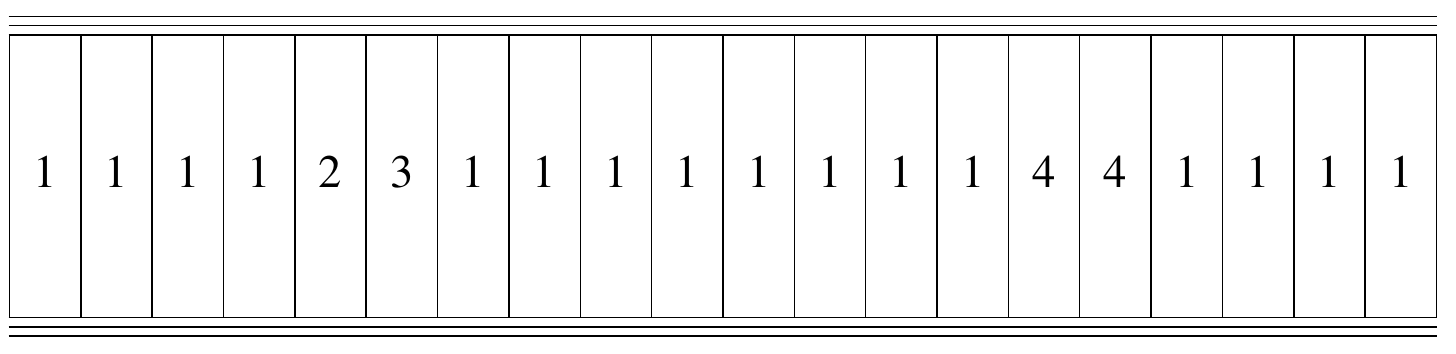
\includegraphics[width=\linewidth]{figures/1D_geometry.png}
\end{figure}

  \begin{columns}
    \column{.5\textwidth}
       \includemedia[addresource=1D_flux_profile.flv, activate=pageopen, deactivate=pageclose, width=5cm, height=5cm, flashvars={source=1D_flux_profile.flv & autoPlay=true & loop=true }]{}{VPlayer.swf}
    \column{.5\textwidth}
      \includemedia[addresource=1D_power_profile.flv, activate=pageopen, deactivate=pageclose, width=5cm, height=5cm, flashvars={source=1D_power_profile.flv & autoPlay=true & loop=true }]{}{VPlayer.swf}
  \end{columns}
  
%\begin{block}{}
%\bi
%\item Control rod withdrawal in regions 2 and 3
%\item Control rod insertion in region 4
%\ei
%\end{block}

\end{frame}
%-------------------------------------------------------------------

%%-------------------------------------------------------------------
%\begin{frame}{1D Flux and Power Profile}
%
%%\begin{center}
%%\movie[width=5cm,height=4cm,showcontrols=true,poster]{IQS}{1D_flux_profile.avi}
%%\movie[width=5cm,height=4cm,showcontrols=true,poster]{Flux}{1D_power_profile.avi}
%%\end{center}
%\end{frame}
%%-------------------------------------------------------------------

%-------------------------------------------------------------------
\begin{frame}{1D Error Convergence}

\begin{columns}
\column{0.6\textwidth}
\begin{figure}[h]
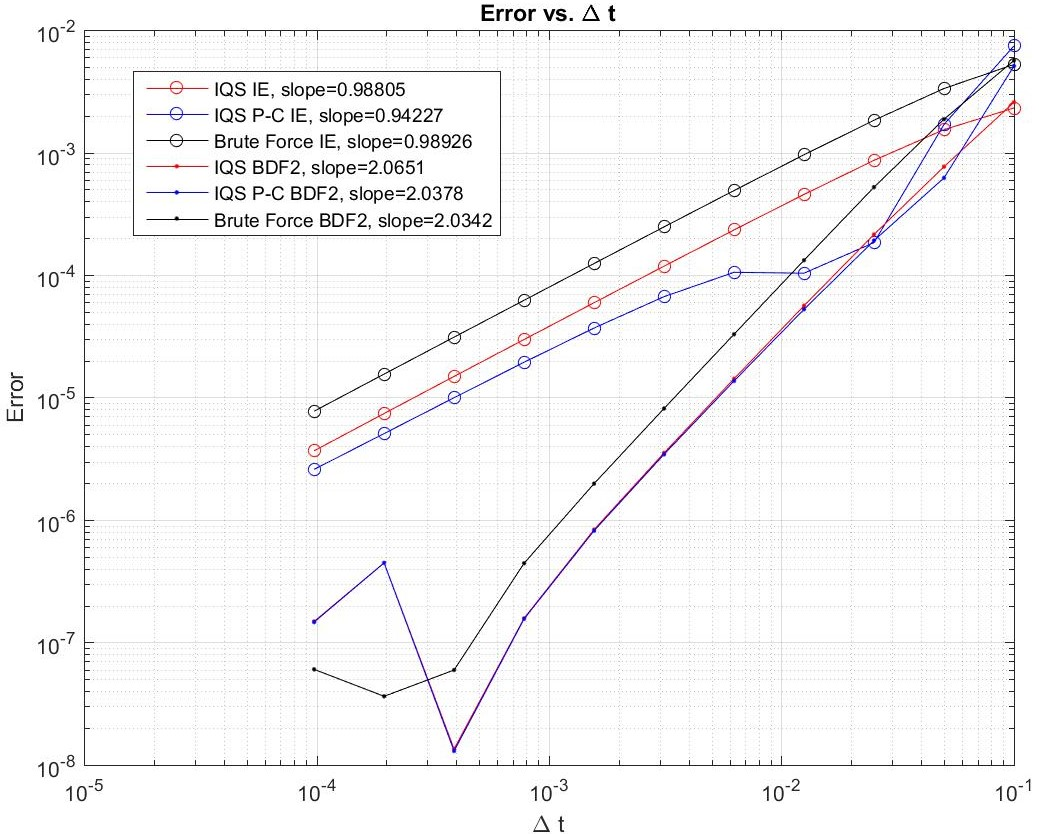
\includegraphics[width=\linewidth]{figures/1D_dt.jpg}
\end{figure}
\column{0.6\textwidth}
\begin{figure}[h]
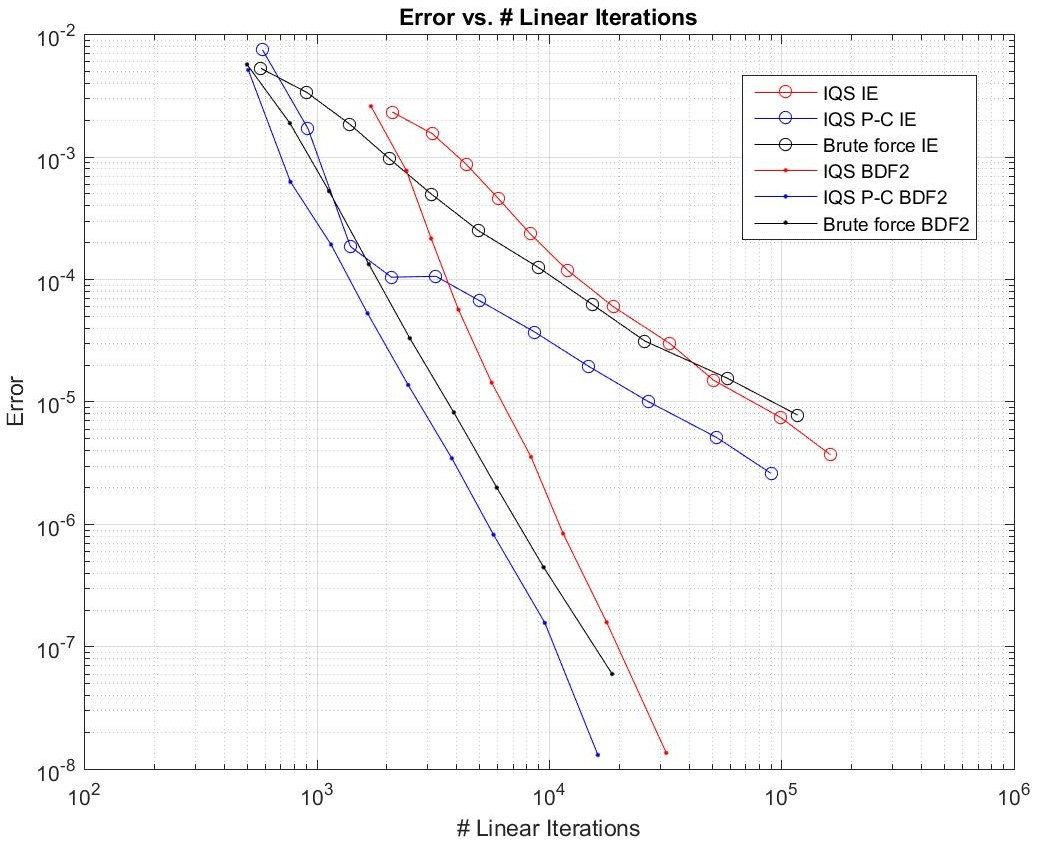
\includegraphics[width=\linewidth]{figures/1D_lin.jpg}
\end{figure}
\end{columns}

\end{frame}
%-------------------------------------------------------------------


%%%%%%%%%%%%%%%%%%%%%%%%%%%%%%%%%%%%%%%%%%%%%%%%%%%%%%%%%%%%%%%%%%%
\subsection{TWIGL Benchmark}
%%%%%%%%%%%%%%%%%%%%%%%%%%%%%%%%%%%%%%%%%%%%%%%%%%%%%%%%%%%%%%%%%%%

%-------------------------------------------------------------------
\begin{frame}{TWIGL Benchmark}
  \begin{columns}
    \column{.5\textwidth}
	\begin{figure}[h]
	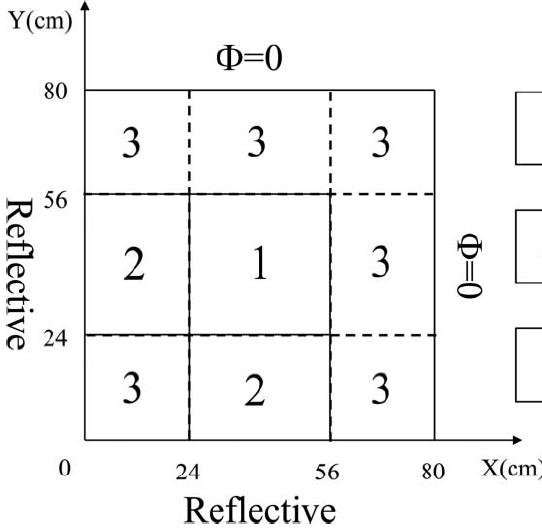
\includegraphics[width=\linewidth]{figures/twigl_geom.png}
	\end{figure}
	\column{0.5\textwidth}
	\includemedia[addresource=TWIGL_flux_profile.flv, activate=pageopen, deactivate=pageclose, width=5cm, height=5cm, flashvars={source=TWIGL_flux_profile.flv & autoPlay=true & loop=true }]{}{VPlayer.swf} \\ \vspace{-20mm}
	\includemedia[addresource=TWIGL_power_profile.flv, activate=pageopen, deactivate=pageclose, width=5cm, height=5cm, flashvars={source=TWIGL_power_profile.flv & autoPlay=true & loop=true }]{}{VPlayer.swf}
  \end{columns}

\end{frame}
%-------------------------------------------------------------------

%-------------------------------------------------------------------
\begin{frame}{TWIGL Error Convergence}

\centering
\begin{figure}[h]
\hspace*{-14mm} 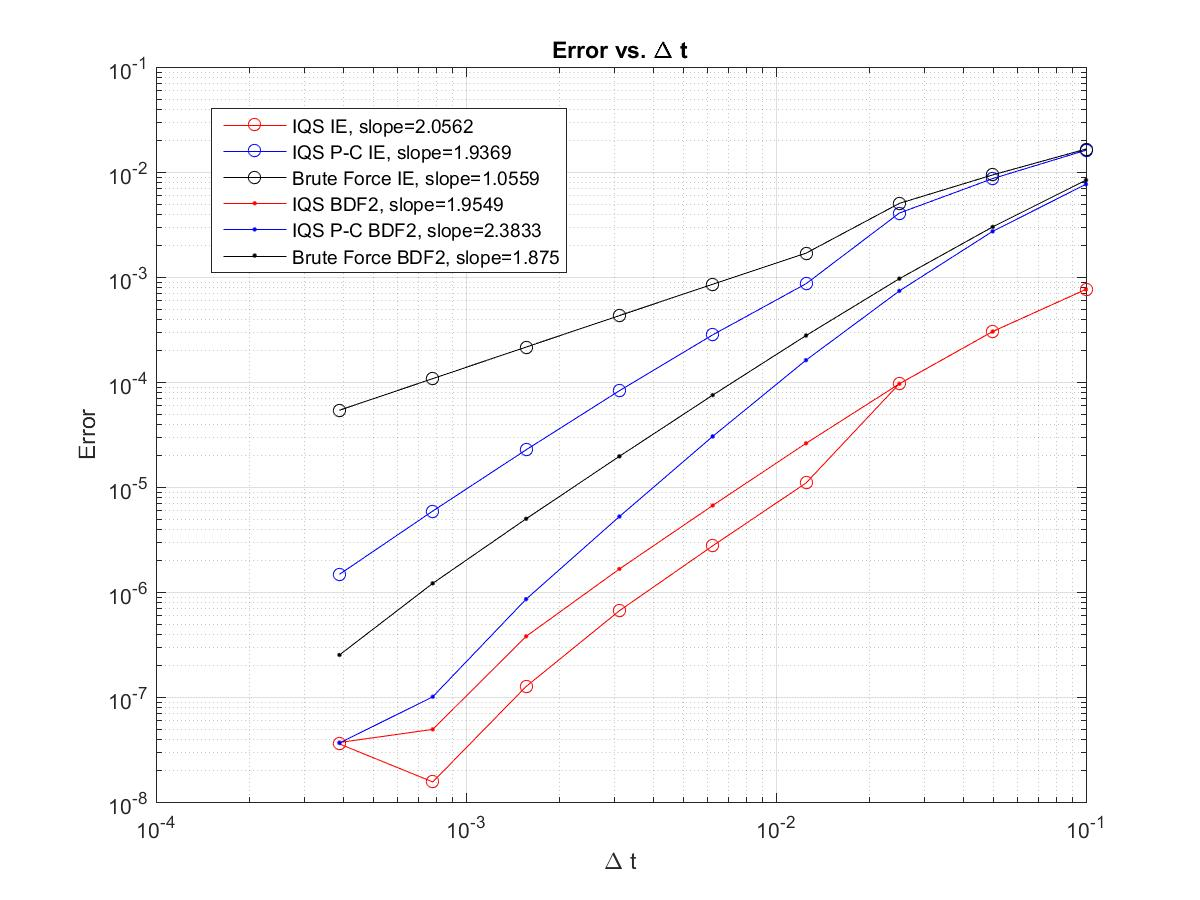
\includegraphics[width=0.55\paperwidth]{figures/TWIGL_ramp_dt.jpg}
\hspace*{-6mm}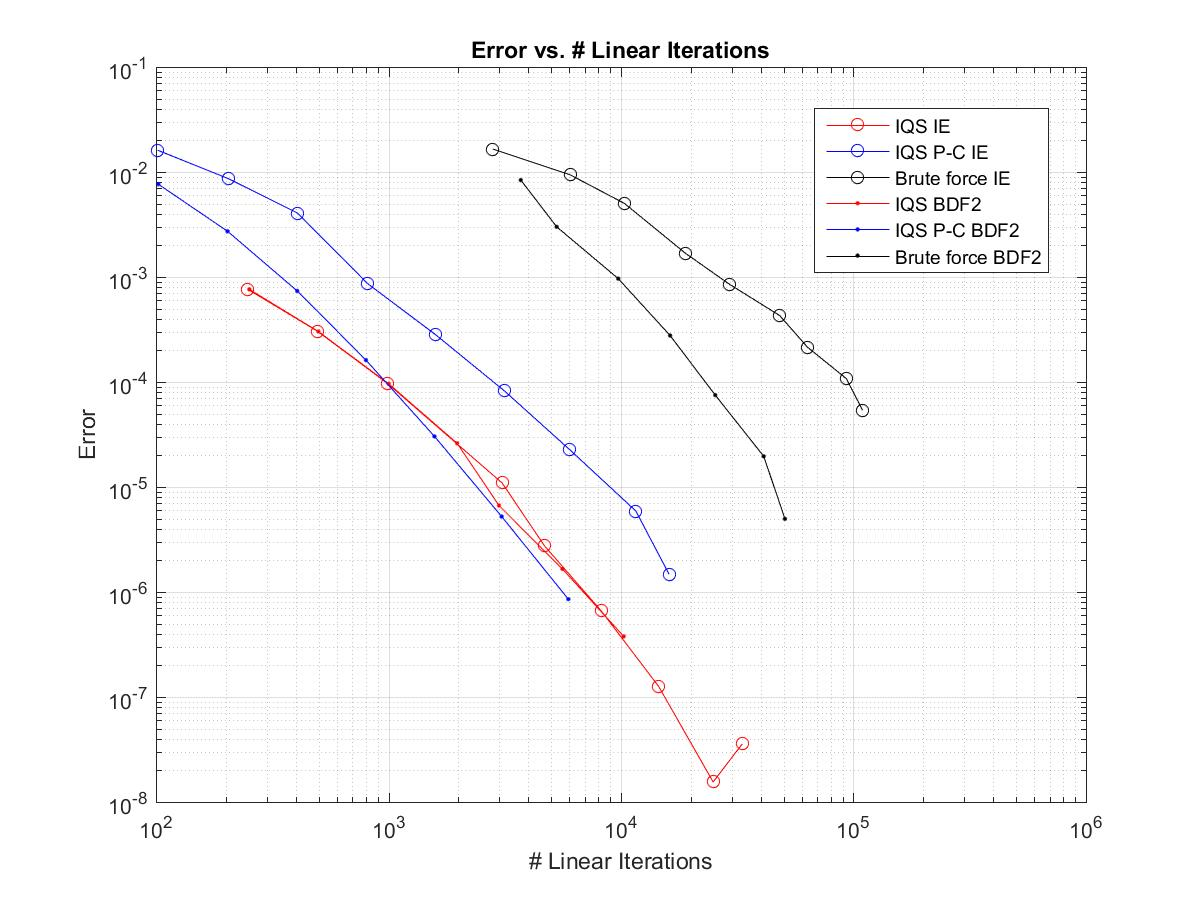
\includegraphics[width=0.55\paperwidth]{figures/TWIGL_ramp_lin.jpg}
\end{figure}

\end{frame}
%-------------------------------------------------------------------

%%%%%%%%%%%%%%%%%%%%%%%%%%%%%%%%%%%%%%%%%%%%%%%%%%%%%%%%%%%%%%%%%%%
\subsection{LRA Benchmark}
%%%%%%%%%%%%%%%%%%%%%%%%%%%%%%%%%%%%%%%%%%%%%%%%%%%%%%%%%%%%%%%%%%%

%-------------------------------------------------------------------
\begin{frame}{LRA Benchmark}

\begin{figure}[h]
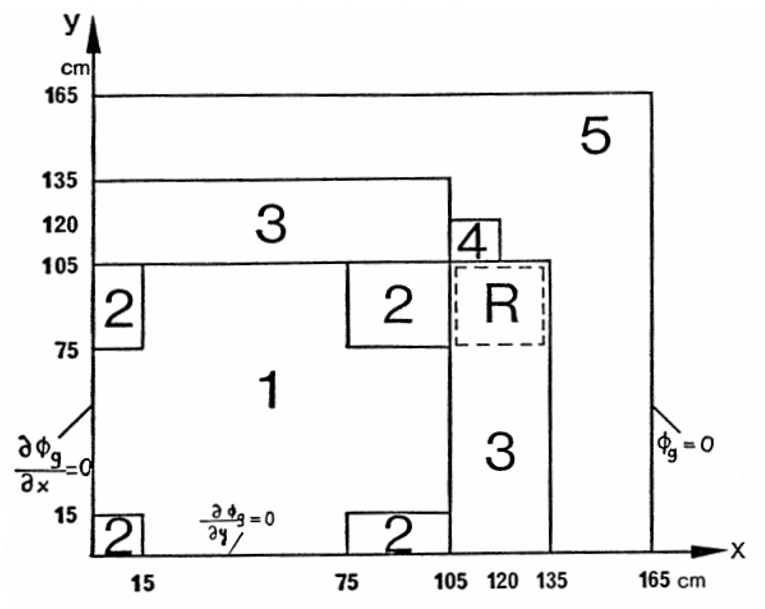
\includegraphics[height=0.8\textheight]{figures/lra_geom.png}
\end{figure}

\end{frame}
%-------------------------------------------------------------------

%-------------------------------------------------------------------
\begin{frame}{LRA Flux, Power, and Temperature Profile}

  \begin{columns}
	\vspace{100mm}
	\column{0.6\textwidth}
	\includemedia[addresource=LRA_flux_profile.flv, activate=pageopen, deactivate=pageclose, width=6cm, height=6cm, flashvars={source=LRA_flux_profile.flv & autoPlay=true & loop=true }]{}{VPlayer.swf}
	\column{0.6\textwidth}
	\includemedia[addresource=LRA_power_profile.flv, activate=pageopen, deactivate=pageclose, width=5cm, height=5cm, flashvars={source=LRA_power_profile.flv & autoPlay=true & loop=true }]{}{VPlayer.swf}
  \end{columns}

\end{frame}
%-------------------------------------------------------------------

%-------------------------------------------------------------------
\begin{frame}{LRA Error Convergence}

\begin{figure}[h]
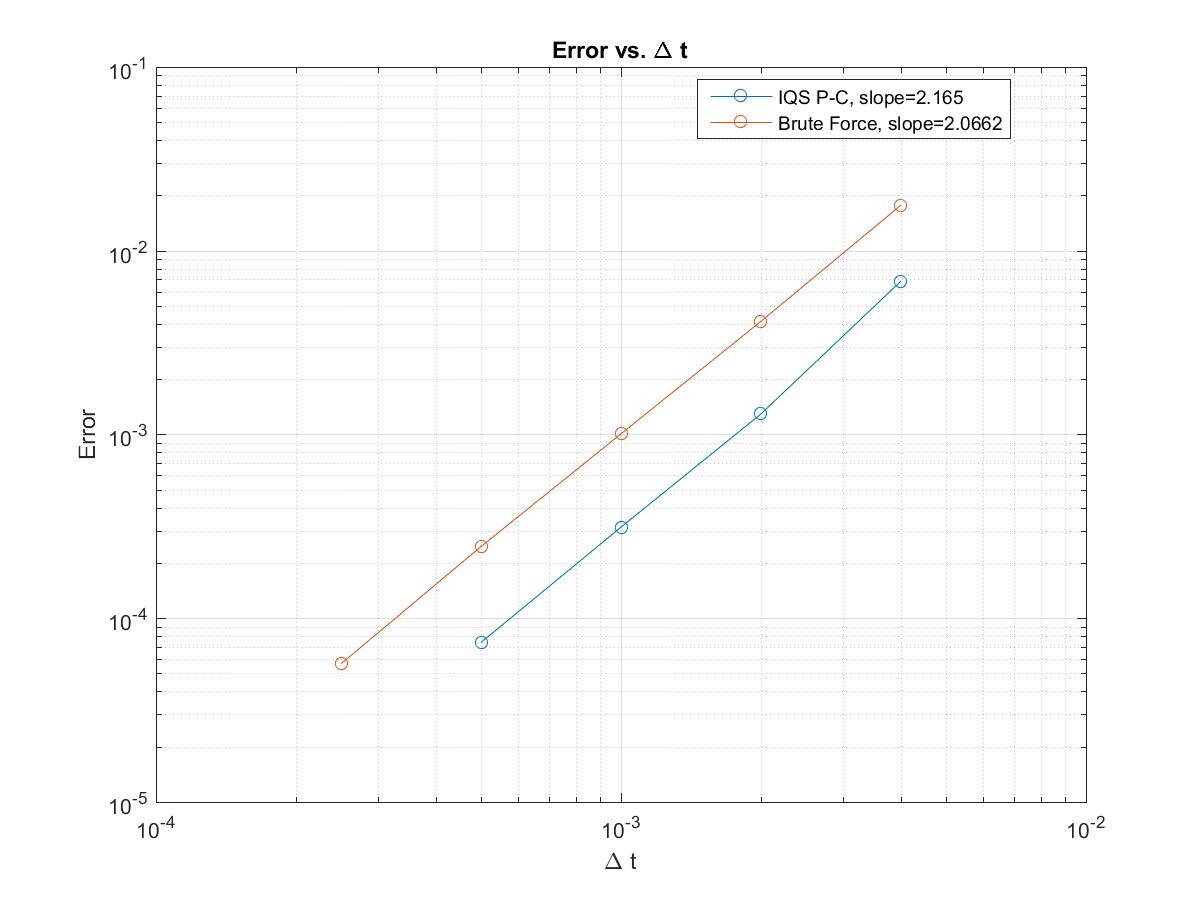
\includegraphics[height=0.8\textheight]{figures/lra_dt.jpg}
\end{figure}

\end{frame}
%-------------------------------------------------------------------

%%%%%%%%%%%%%%%%%%%%%%%%%%%%%%%%%%%%%%%%%%%%%%%%%%%%%%%%%%%%%%%%%%%%%%%%%%%%%%%%%%%%%%%

%{
%\setbeamercolor{background canvas}{bg=}
%\includepdf[pages={9-24}]{./PDT-Scaling-MLA-DH-TS-TST-May14-final.pdf}
%\includepdf[pages={26}]{./PDT-Scaling-MLA-DH-TS-TST-May14-final.pdf}
%}

%%%%%%%%%%%%%%%%%%%%%%%%%%%%%%%%%%%%%%%%%%%%%%%%%%%%%%%%%%%%%%%%%%%%%

%{
%\setbeamercolor{background canvas}{bg=}
%\includepdf[pages={-}]{./RagusaPresentationV3-Copy.pdf}
%}

%%%%%%%%%%%%%%%%%%%%%%%%%%%%%%%%%%%%%%%%%%%%%%%%%%%%%%%%%%%%%%%%%%%%%

%%%%%%%%%%%%%%%%%%%%%%%%%%%%%%%%%%%%%%%%%%%%%%%%%%%%%%%%%%%%%%%%%%%%%
%%%%%%%%%%%%%%%%%%%%%%%%%%%%%%%%%%%%%%%%%%%%%%%%%%%%%%%%%%%%%%%%%%%%%
\section{Wrap-up}
%%%%%%%%%%%%%%%%%%%%%%%%%%%%%%%%%%%%%%%%%%%%%%%%%%%%%%%%%%%%%%%%%%%%%
%%%%%%%%%%%%%%%%%%%%%%%%%%%%%%%%%%%%%%%%%%%%%%%%%%%%%%%%%%%%%%%%%%%%%

%-------------------------------------------------------------------
\begin{frame}{Conclusion and Outlook}

\begin{block}{Completed}
\bi
\item Complete IQS and IQS P-C Implementation in Rattlesnake
\item 1D Test case to verify error convergence
\item TWIGL kinetics  benchmark (neutronics only)
\item LRA dynamics benchmark (temperature feedback)
\ei
\end{block}

\begin{block}{In progress}
\bi
\item Time step adaptation/control
\ei
\end{block}
\begin{block}{Next Steps}
\bi
\item DFEM Diffusion action system
\item DFEM SN Transport action system
\item More benchmarks (LMW, TREAT, etc.)
\item Study of a JFNK-based algorithm to resolve the IQS nonlinearity between the \tcr{amplitude}/\tcb{shape} equations
\ei
\end{block}

\end{frame}
%-------------------------------------------------------------------

%-------------------------------------------------------------------
\begin{frame}{Questions ?}


\begin{block}{Thanks}
\begin{itemize}
\item Mark DeHart (INL, TREAT M\&S lead)
\item NEAMS
\end{itemize}

\begin{block}{}
\begin{figure}
	When you realize you sent the same job 100 times to Falcon:
	\centering
	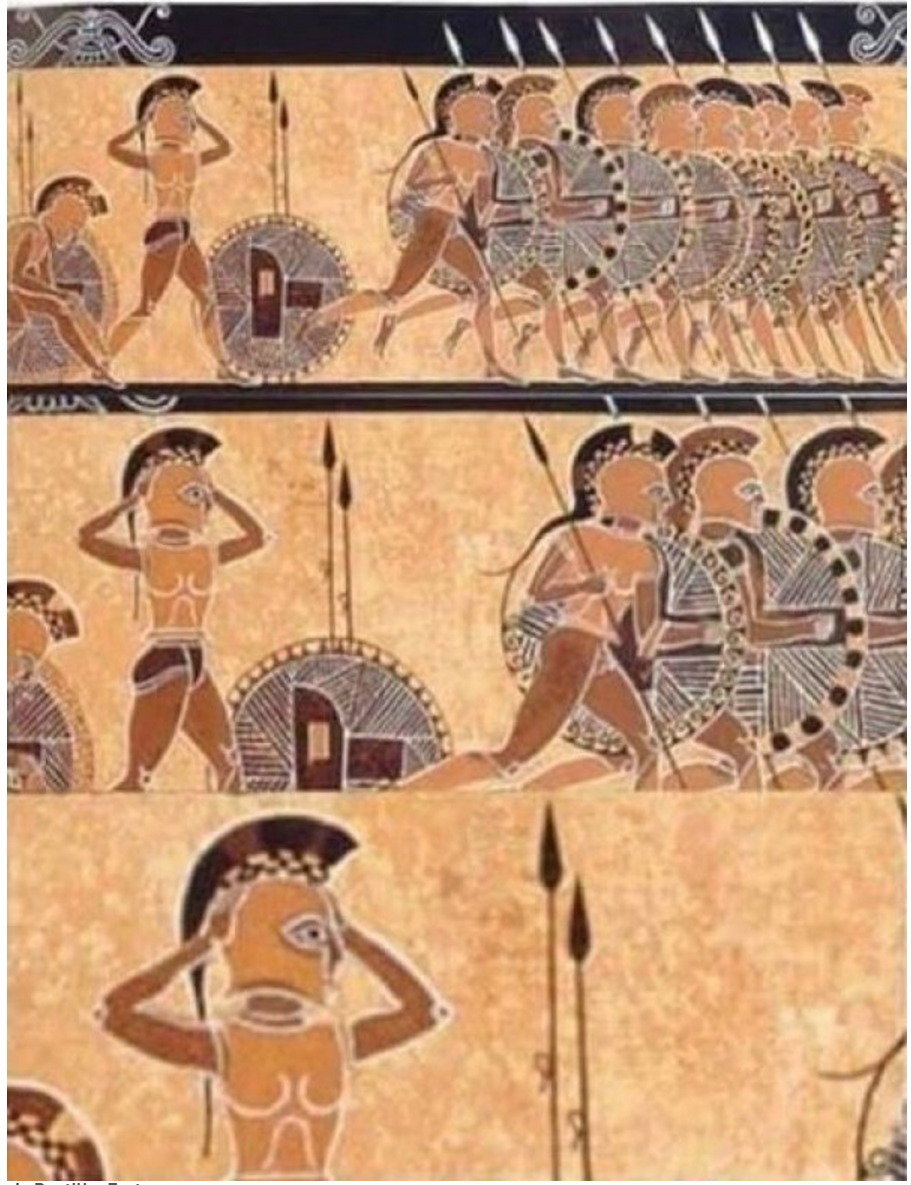
\includegraphics[scale=0.25]{./final_fig.png}
\end{figure}
\end{block}

\end{block}

\end{frame}
%-------------------------------------------------------------------


%%-------------------------------------------------------------------
%\begin{frame}{}
%
%
%\begin{block}{}
%\end{block}
%
%\end{frame}
%%-------------------------------------------------------------------

%%%%%%%%%%%%%%%%%%%%%%%%%%%%%%%%%%%%%%%%%%%%%%%%%%%%%%%%%%%%%%%%%%%%
%%%%%%%%%%%%%%%%%%%%%%%%%%%%%%%%%%%%%%%%%%%%%%%%%%%%%%%%%%%%%%%%%%%%
%\begin{frame}{Thank you}
%
%\begin{block}{Computational Transport}
%\begin{figure}
%	\centering
%	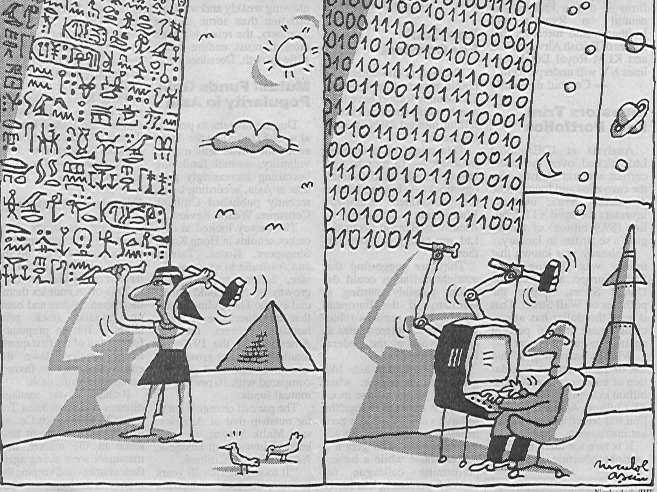
\includegraphics[scale=0.33]{./fig/crunching.png}
%\end{figure}
%\end{block}
%
%\end{frame}
%%%%%%%%%%%%%%%%%%%%%%%%%%%%%%%%%%%%%%%%%%%%%%%%%%%%%%%%%%%%%%%%%%%%
%%%%%%%%%%%%%%%%%%%%%%%%%%%%%%%%%%%%%%%%%%%%%%%%%%%%%%%%%%%%%%%%%%%%

%************************************************

\end{document}